%%%%%%%%%%%%%%%%%%%%%%%%%%%%%%%%%%%%%%%%%%%%%%%%%%%
%%%%%%%%%%%%%%%教案头%%%%%%%%%%%%%%%%%%%%%%%%%%%%%%%
%%%%%%%%%%%%%%%%%%%%%%%%%%%%%%%%%%%%%%%%%%%%%%%%%%%
\mode <article>{

\begin{longtable}{|m{20mm}|m{20mm}|m{20mm}|m{20mm}|m{20mm}|m{28mm}|}
\caption*{\huge 教案头}\\
\hline
\endfirsthead
\multicolumn{6}{l}{(续表)}\\
\hline
\endhead
\hline
\multicolumn{6}{l}{\itshape 接下一页表格.......}\\ [2ex]
\endfoot
\hline
\endlastfoot
\centering{授课单元}&\multicolumn{3}{m{60mm}|}{\centering 电动机正反转间歇运行控制}&\centering{授课日期}&2014年03月12日 \\
\hline
\centering 授课地点 & \multicolumn{3}{m{60mm}|}{B4-209}&\centering 授课学时 & 2 \\
\hline
& \multicolumn{2}{m{40mm}|}{能力目标} & \multicolumn{2}{m{40mm}|}{知识目标}&素质目标 \\
\cline{2-6}
\centering 教学目标&\multicolumn{2}{m{40mm}|}{\begin{enumerate}
\item 能够运用互锁 PLC 程序实现电动机的正反间歇运转控制
\item 能够运用定时器实现电动机运转的间歇运转控制
\item 能够根据控制要求进行系统I/O分配
\end{enumerate}} &\multicolumn{2}{m{40mm}|}{\begin{enumerate}
\item 掌握互锁程序的设计方法
\item 掌握程序流程图的绘制方法
\end{enumerate}} & {能够进行故障分析,以培养问题分析能力}\\
\hline
\centering 能力训练任务或案例 &\multicolumn{5}{m{108mm}|}{\begin{enumerate}
\item 编制电动机正反间歇运转控制I/o分配表
\item 设计电动机正反间歇运转PLC控制程序
\item PLC控制接线
\item PLC控制程序输入
\item PLC控制检验
\end{enumerate}}\\
\hline
\centering 教学重点 & \multicolumn{5}{m{108mm}|}{正反转互锁控制程序的设计}\\
\hline
\centering 教学难点与解决办法 &\multicolumn{5}{m{108mm}|}{难点:具有互锁功能的PLC程序编写。解决方法:通过指令演示使学生了解并掌握时间指令的基本结构}\\
\hline
\centering 德育内容 &\multicolumn{5}{m{108mm}|}{无}\\
\hline
 &教材 & \multicolumn{4}{l|}{PLC技术}\\
\cline{2-6}& 教学资源 &\multicolumn{4}{m{88mm}|}{PPT}\\
\cline{2-6}\centering 使用的教学材料& 主要教学仪器设备和工具等 &\multicolumn{4}{m{88mm}|}{投影机、西门子PLC编程控制台、万用表、螺丝刀}\\
\cline{2-6}& 主要耗材 &\multicolumn{4}{m{88mm}|}{\qquad}\\
\hline
\centering 教学模式 &\multicolumn{2}{l|}{项目化}&\centering 教学手段 &\multicolumn{2}{l|}{项目化}\\
\hline
\centering 学生成果与过程考核方式 &\multicolumn{5}{m{108mm}|}{成果:具有报警功能的电动机单向连续运行PLC控制程序、控制程序I/O分配表、电动机控制接线。考核方式:对项目完成情况进行评分,作为该项目考核结果}
\end{longtable}
\clearpage

%%%%%%%%%%%%%%%%%%%%%%%%%%%%%%%%%%%%%%%%%%%%%%%%%%%%%
%%%%%%%%%%%%%%%教学实施过程%%%%%%%%%%%%%%%%%%%%%%%%%%%%
%%%%%%%%%%%%%%%%%%%%%%%%%%%%%%%%%%%%%%%%%%%%%%%%%%%%%

\begin{landscape}
\begin{longtable}{|m{10mm}|m{50mm}|m{50mm}|m{50mm}|m{15mm}|}
\caption*{\huge 教学组织与实施}\\
\hline
\endfirsthead
\multicolumn{5}{l}{\small 接上页}\\
\hline
\multicolumn{1}{|c|}{步骤}&\multicolumn{1}{c|}{教学内容}&\multicolumn{1}{c|}{教师活动}&\multicolumn{1}{c|}{学生活动}&\multicolumn{1}{c|}{时间}\\
\hline
\endhead

\multicolumn{5}{r}{\small 接下页}\\
\endfoot
\hline
\endlastfoot
\multicolumn{1}{|c|}{步骤}&\multicolumn{1}{c|}{教学内容}&\multicolumn{1}{c|}{教师活动}&\multicolumn{1}{c|}{学生活动}&\multicolumn{1}{c|}{时间}\\\hline
引入&\begin{enumerate}
\item 具有正反间歇运转功能的电动机控制
\end{enumerate} &\begin{enumerate}
\item 介绍项目情景
\item 讲述控制要求
\item 布置编制I/O分配表和程序流程图任务
\end{enumerate} &\begin{enumerate}
\item 学生记录控制要求
\item 学生领取项目任务
\end{enumerate} &5 \\\hline
设计&
\begin{enumerate}
\item 编制电动控制I/O分配表和程序流程图
\end{enumerate} &\begin{enumerate}
\item 了解学生编制I/O分配表和程序流程图的情况
\end{enumerate} &\begin{enumerate}
\item 学生编制I/O分配表和程序流程图
\item 学生展示编制的I/O分配表和程序流程图
\end{enumerate} &10 \\\hline
设计&\begin{enumerate}
\item 设计具有正反间歇运转功能的电动机PLC控制程序
\end{enumerate}
&\begin{enumerate}
\item 指导学生进行PLC控制程序设计
\end{enumerate} &\begin{enumerate}
\item 学生设计PLC程序
\end{enumerate} &20 \\\hline
操作&
\begin{enumerate}
\item PLC控制接线
\end{enumerate} &\begin{enumerate}
\item 教师指导学生进行PLC控制接线
\item 教师收集学生接线过程中存在的问题
\end{enumerate} &\begin{enumerate}
\item 学生根据设计进行PLC控制接线
\end{enumerate} &10 \\\hline
编程&
\begin{enumerate}
\item 编写电机控制PLC程序
\end{enumerate} &\begin{enumerate}
\item 指导学生编写PLC程序
\end{enumerate} &\begin{enumerate}
\item 学生根据设计编写PLC程序
\end{enumerate} &25 \\\hline
\centering 检验修改&\begin{enumerate}
\item 检验电动PLC控制程序的正确性
\end{enumerate}&\begin{enumerate}
\item 教师收集PLC控制程序存在的问题
\item 教师指导学生进行程序验证
\item 教师展示出错程序
\item 总结错误原因
\end{enumerate}&\begin{enumerate}
\item 学生进行PLC控制程序的控制验证,并记录结果
\item 学生讨论出错原因
\item 学生根据验证情况修改PLC控制程序
\end{enumerate}&15 \\\hline
\centering 本次课总结(评价)&\begin{enumerate}
\item 总结互锁PLC程序的基本结构 
\end{enumerate}&总结互锁PLC程序的基本结构  &学生倾听记录 &5 \\\hline
\centering 学生学习笔记或工单等检查情况&\multicolumn{4}{m{165mm}|}{\quad}\\\hline
\centering 课后作业&\multicolumn{4}{m{165mm}|}{}\\\hline
\centering 教学体会&\multicolumn{4}{m{165mm}|}{\quad}\\
\end{longtable}

\end{landscape}
\clearpage

%%%%%%%%%%%%%%%%%%%%%%%%%%%%%%%%%%%%%%%%%%%%%%%%%%%%
%%%%%%%%%%%%%%%%%%%%板书设计%%%%%%%%%%%%%%%%%%%%%%%%%
%%%%%%%%%%%%%%%%%%%%%%%%%%%%%%%%%%%%%%%%%%%%%%%%%%%%
\lecture{计算机控制系统简介}{yinlun}
\begin{center}
{\huge 板书设计}
\end{center}
}

\mode<presentation>{ \section{电动机正反转间歇转控制} }
\begin{frame}[containsverbatim]{电动机正反转间歇转控制}
\begin{block}{控制要求}
\begin{itemize}
\item 按下SB1按钮,三相电动机开始正转。
\item 正转5min后,停3min,然后开始反转。
\item 反转5min后,停5min,再正转,依次循环。
\item 按下SB2按钮,三相电动机停止转动。
\item 当电动机过载时,过载保护器FR断开,三相电动机停止运转。
\end{itemize}
\end{block}
\end{frame}
\begin{frame}{}
\begin{block}{工作任务}
\begin{itemize}
\item 编制I/O配置表
\item 设计电动机PLC控制程序
\item 电动机控制接线
\item 控制程序录入
\item 控制检查与修正
\end{itemize}
\end{block}
\end{frame}
\begin{frame}
\begin{block}{I/O分配表}
\begin{small}
\begin{tabular}{|c|c|c|c|c|c|}
\hline 
\multicolumn{2}{|c|}{输入设备} & PLC &\multicolumn{2}{|c|}{输出设备} & PLC \\ 
\cline{1-2}\cline{4-5}
代号 & 功能 & 输入 & 代号 & 功能 & 输出 \\ 
\hline 
SB1 & 启动按钮 & I0.0 & KM1 & 正转接触器 & Q0.0 \\ 
\hline 
SB2 & 停止按钮 & I0.1 & KM2 & 反转接触器& Q0.1 \\ 
\hline 
FR & 过载保护 & I0.2 &  &  &  \\ 
\hline
\end{tabular} 
\end{small}
\end{block}
\end{frame}
\begin{frame}{总结}
\begin{block}{互锁PLC程序}
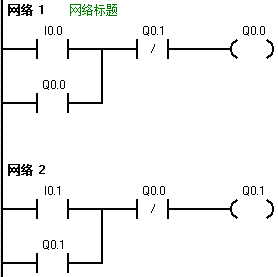
\includegraphics[scale=0.95]{fusuoPLC.png}
\end{block}
\end{frame}
\endinput